%!TEX program=xelatex

\documentclass[11pt]{ctexart}  
\usepackage[top=2cm, bottom=2cm, left=2cm, right=2cm]{geometry}  
\usepackage{algorithm}  
\usepackage{algorithmicx}  
\usepackage{algpseudocode}  
\usepackage{amsmath}  
\usepackage{graphicx}
\usepackage{amsmath}
\usepackage{amssymb}


\floatname{algorithm}{算法}
\renewcommand{\algorithmicrequire}{\textbf{输入:}}  
\renewcommand{\algorithmicensure}{\textbf{输出:}} 

\title{密码学实验报告1}
\author{张天辰	17377321}


\begin{document}
\maketitle{}



\section{Eratosthenes筛法}
\subsection{递归算法基本原理}
为求$1 \sim n$的所有素数,可采用如下方法:先求出$1 \sim \sqrt n$中所有素数,再把这些素数的倍数删去,留下的数就是$1 \sim n$中所有素数。依照这样的算法进行递归,可以设置一个递归出口,即在$n < 10$时直接给出相应的素数。
\subsection{算法实现}
\begin{algorithm}  
    \caption{递归Eratosthenes筛法}  
    \begin{algorithmic}[1] %每行显示行号  
        \Require 数字上限$n$  
        \Ensure $1 \sim n$范围内所有的素数  
        \Function {badEratosthenes}{$n$} 
            \State $standard = [2, 3, 5, 7]$
            \If {n < 10}
                \State \Return $p in standard: p \leqslant n$
            \Else
                \State $primes \gets $\Call{badEratosthenes}{$[\sqrt n]$}
                \State $flag[1, 2, \; \cdots \; ,n] \gets False$
                \For {each p in primes}
                    \State $j \gets 2 * p$
                    \While {$j \leqslant n$}
                        \State $flag[j] \gets True$
                        \State $j \gets j + p$
                    \EndWhile
                \EndFor
                \State \Return $[p: flag[p] == False]$
            \EndIf
        \EndFunction  
    \end{algorithmic}  
\end{algorithm} 
\subsection{优化后的算法}
递归算法进行了过多的重复计算。为此不再使用递归算法,而是把从$2$开始,把表中$2$的倍数删去,再找到下一个元素$3$,把其倍数删去,直到找到$\sqrt n$位置。每次把$i$的倍数删去时,可从$i^2$开始,因为小于$i^2$的$i$的倍数一定有小于$i$的素因子,因此已经被删去。
\begin{algorithm}  
    \caption{优化Eratosthenes筛法}  
    \begin{algorithmic}[1] %每行显示行号  
        \Require 数字上限$n$  
        \Ensure $1 \sim n$范围内所有的素数  
        \Function {Eratosthenes}{$n$}  
            \State $flag[1...n] \gets {False}$  
            \For {each $i\in [2, [\sqrt{n}]]$}
            	\If {$flag[i] == False$}
            		\State $j \gets i * i$
            		\While {$j \leqslant n$}
            			\State $flag[i] \gets {True}$
            			\State $j \gets j + i$
            		\EndWhile
            	\EndIf
            \EndFor
            \State \Return $[p: flag[p] == False]$
        \EndFunction  
    \end{algorithmic}  
\end{algorithm} 
\subsection{复杂度分析}
在对素数$p$的倍数进行删除时,内层代码执行了$\frac{n}{p} - 1$次,因此总消耗为:
$$\sum_{p \leqslant \sqrt n} \frac{n}{p} - 1 = n\sum_{p \leqslant \sqrt n} \frac{1}{p} - \pi(n)$$
其中$\pi(n)$表示不超过$n$的素数个数。根据素数定理,$\pi(n) = O(\frac{n}{\ln n})$
由Mertens第二定理:
$$\lim_{x \to \infty}\sum_{p \leqslant \sqrt n}\frac{1}{p} - \ln \ln n = M$$
其中$M$是Meissel-Mertens常数,约为$0.26$。因此时间复杂度为$O(n\log \log n)$
对算法进行上述优化不会影响复杂度。空间复杂度为$O(n)$。
\newpage
\subsection{再次优化——欧拉筛}
欧拉筛算法为让每个合数只被其最小素因子筛一次,从而不重复筛选。此时,时间复杂度被优化为$O(n)$。算法如下:
\begin{algorithm}  
    \caption{Euler筛法}  
    \begin{algorithmic}[1] %每行显示行号  
        \Require 数字上限$n$  
        \Ensure $1 \sim n$范围内所有的素数  
        \Function {Euler}{$n$} 
            \State $primes \gets []$ 
            \State $flag[1...n] \gets {True}$  
            \For {each $i\in [2, n]$}
                \If {$flag[i] == True$}
                    \State $primes.append(i)$
                \EndIf
                \For {each p in primes}
                    \If {$i * p < n$}
                        \State Break
                    \EndIf
                    \State $flag[i * p] \gets False$
                    \If {$i \% p == 0$}
                        \State Break
                    \EndIf
                \EndFor
            \EndFor
            \State \Return $primes$
        \EndFunction  
    \end{algorithmic}  
\end{algorithm} 
如果$i$是$prime[j]$的倍数,则设$i = k \times prime[j]$,$i \times prime[j + 1] = prime[j] \times k \times prime[j + 1]$,当$i = k \times prime[j + 1]$时删去,因此算法到此就跳出循环。
\newpage{}
\subsection{测试样例}
先验证算法正确性,见图\ref{img_sieve1}。
\begin{figure}[htbp]
\centering
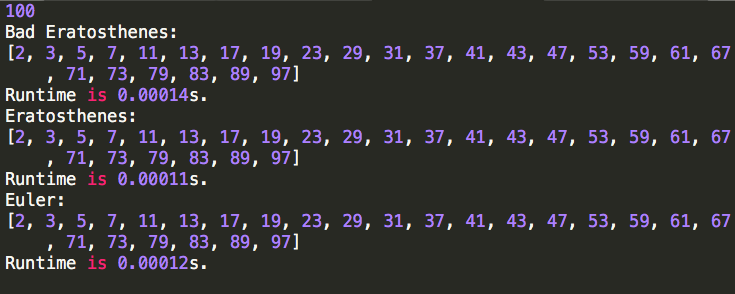
\includegraphics[height=4.41cm,width=11.02cm]{sieve_small.png}
\caption{筛法}
\label{img_sieve1}
\end{figure}
在确认正确性后,为节省时间不再输出结果,只比较时间,见图\ref{img_Sieve2}
\begin{figure}[htbp]
\centering
\includegraphics[height=4.98cm,width=7.17cm]{Sieve_big.png}
\caption{筛法(大数)}
\label{img_Sieve2}
\end{figure}

\section{Euclid算法}

\subsection{Euclid算法原理}
Euclid算法又称为辗转相除法,是一种求最大公因数的方法。其算法设计基于如下事实:若$a/b$的带余除法写成如下形式
$$a = q \times b + r$$
则有
$$gcd(a,b) = gcd(b,r)$$
如此可将除法规模不断缩小,以达到求最大公因子的目的。
\newpage{}
\subsection{算法实现}
\begin{algorithm}  
    \caption{Euclid算法}  
    \begin{algorithmic}[1] %每行显示行号  
        \Require $num1$, $num2$ 
        \Ensure $gcd(num1,num2)$  
        \Function {Euclid}{$num1,num2$}
            \If {num1 < num2}   
                \State $num1, num2 \gets num2, num1$
            \EndIf
            \While {$num1 \% num2 \neq 0$}
                \State $a, b = b, num1 \% num2$
            \EndWhile
            \State \Return $num2$
        \EndFunction  
    \end{algorithmic}  
\end{algorithm} 

\subsection{算法复杂度分析}
显然,该算法空间复杂度为$O(1)$,下面分析时间复杂度:

不妨设输入的两个数为$a$和$b$,$a\geqslant b$,并设需要做$n$次除法。
令$r_0 = a, r_1 = b$。则:
$$r_0 = q_1r_1 + r_2\quad r_1 = q_2r_2 + r_3 \quad \cdots \quad r_{n - 1} = q_nr_n $$
容易发现$$q_1, q_2, q_3,\quad \cdots \quad q_{n - 1} \geqslant 1, q_n \geqslant 2$$
则
$$r_n \geqslant 1 = f_2 \quad r_{n - 1} \geqslant 2r_n \geqslant 2f_2 = f_3 \quad r_{n-2} \geqslant f_2 + f_3 = f_4\quad \cdots$$
其中$f_n$表示Fibonacci数列第$n$项。故
$$r_1 \geqslant f_{n + 1} > \alpha^{n - 1}$$
其中$\alpha = \frac{\sqrt{5} - 1}{2}$。因此
$$\lg r_1 = \lg b > \lg \alpha^{n - 1} > \frac{n - 1}{5}$$
所以
$$n \leqslant 5\lg r_1 = 5\lg b$$
因此Euclid算法的时间复杂度为$O(\lg min{a, b})$

\subsection{扩展Euclid算法}
B\'ezout定理给出,对于任意整数$a, b$,总存在整数$s, t$,使得$sa + tb = gcd(a, b)$。Euclid算法并不能给出如上的线性系数$s, t$,但只需将算法稍作优化,便得到可以同时得到最大公因子和上述线性系数的扩展Euclid算法。

实现线性系数的求解可以有两种方法:一种是在递归求解最大公因子后回溯求解系数;另一种是在循环时直接计算系数,其原理如下:
令$r_{-1} = a, r_0 = b$
$$r_{i - 2} = q_i r_{i - 1} + r_i\quad i = 1, 2, \; \cdots \;,n$$
设$r_i = a x_i + b y_i$
可推出
$$x_i = x_{i - 2} - q_i x_{i - 1} \quad y_i = y_{i - 2} - q_i y_{i - 1}$$
\subsection{扩展算法实现}
\begin{algorithm}  
    \caption{Euclid算法回溯}  
    \begin{algorithmic}[1] %每行显示行号  
        \Require $num1, num2$  
        \Ensure $gcd(num1, num2)$,线性系数$coe1, coe2$  
        \Function {backEuclid}{$num1, num2$} 
            \If{num1 < num2}
                \State $change \gets True$
                \State $big, small \gets num2, num1$
            \Else
                \State $change \gets False$
                \State $big, small \gets num1, num2$
            \EndIf
            \If {small == 0}
                \State \Return $big, 1, 0$
            \Else
                \State $rest, coeBig_n, coeSmall_n \gets$ \Call{backEuclid}{$small, big \% small$}
                \State $coeBig \gets coeSmall_n$
                \State $coeSmall \gets coeBig_n - coeSmall_n * [big / small]$
                \If{change == True}
                    \State \Return $rest, coeSmall, coeBig$
                \Else
                    \State \Return $rest, coeBig, coeSmall$
                \EndIf 
            \EndIf  
        \EndFunction  
    \end{algorithmic}  
\end{algorithm} 
\newpage{}
\begin{algorithm}  
    \caption{扩展Euclid算法}  
    \begin{algorithmic}[1] %每行显示行号  
        \Require $num1, num2$  
        \Ensure $gcd(num1, num2)$,线性系数$coe1, coe2$  
        \Function {extendEuclid}{$num1, num2$} 
            \If{num1 < num2}
                \State $change \gets True$
                \State $big, small \gets num2, num1$
            \Else
                \State $change \gets False$
                \State $big, small \gets num1, num2$
            \EndIf
            \State $rest, coeBig, coeSmall \gets big, 1, 0$
            \State $rest_n, coeBig_n, coeSmall_n \gets small, 1, 0$
            \While {$rest_n \neq 0$}
                \State $q \gets rest // rest_n$
                \State $temp1 \gets rest - q * rest_n$
                \State $temp2 \gets coeBig - q * coeBig_n$
                \State $temp1 \gets coeSmall - q * coeSmall_n$
                \State $rest, coeBig, coeSmall \gets rest_n, coeBig_n, coeSmall_n$
                \State $rest_n, coeBig_n, coeSmall_n \gets temp1, temp2, temp3$
            \EndWhile
            \If{change == True}
                \State \Return $rest, coeSmall, coeBig$
            \Else
                \State \Return $rest, coeBig, coeSmall$
            \EndIf
        \EndFunction  
    \end{algorithmic}  
\end{algorithm} 
\subsection{两种算法比较}
回溯算法和扩展算法的时间复杂度相仿,均与普通欧几里得算法相同。但是因为回溯算法需要递归调用函数,因此比使用循环的算法需要更多的时间。在空间方面,递归算法也较为劣势,每次递归都要开辟另外的空间,复杂度为$O(min{a, b})$;而扩展算法复杂度为$O(1)$。
\newpage{}
\subsection{测试案例}
\begin{figure}[htbp]
\centering
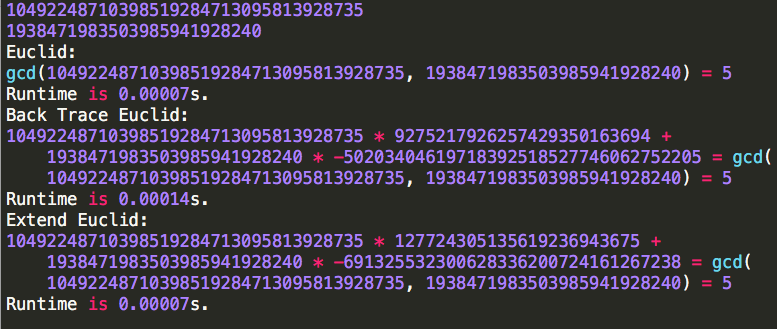
\includegraphics[height=4.93cm,width=11.65cm]{Euclid.png}
\caption{Euclid算法}
\label{img_Euclid}
\end{figure}

\section{快速模幂算法}

\subsection{基本流程}
快速模幂算法又称为“平方乘算法”。顾名思义,算法基本由平方操作和乘操作两部分组成。首先,将指数写成二进制的形式。此后,从二进制指数的高位向低位遍历,如果遇到0,就将目前的结果平方后取模;否则就在平方后再模乘上原始底数。如此操作的原理是容易在数学上验证的。因为平方操作相当于把二进制指数左移一位,也就相当于在右侧加0。如果再乘上原始底数,就相当于在右侧加1。这样的算法避免了暴力算法的逐次模乘,大大提高了效率。


\subsection{算法实现}
\begin{algorithm}  
    \caption{暴力模幂算法}  
    \begin{algorithmic}[1] %每行显示行号  
        \Require 底数$base$, 指数$power$, 模$mod$  
        \Ensure $base^{power}\quad$(mod $mod$)  
        \Function {modPower}{$base, power, mod$}   
            \State $result \gets 1$
            \For {each $i\in [1, power]$}
                \State $result \gets (result * base)\quad\% mod$
            \EndFor
            \State \Return $result$
        \EndFunction  
    \end{algorithmic}  
\end{algorithm} 
\begin{algorithm}  
    \caption{快速模幂算法}  
    \begin{algorithmic}[1] %每行显示行号  
        \Require 底数$base$, 指数$power$, 模$mod$  
        \Ensure $base^{power}\quad$(mod $mod$)  
        \Function {modPower}{$base, power, mod$}  
            \State $binary[] \gets bin(power)$  
            \State $result \gets 1$
            \For {each $i\in binary$}
            	\If {$i == '0'$}
            		\State $result \gets result^2 \quad\% mod$
            	\Else
            		\State $result \gets result^2 \quad\% mod$
            		\State $result \gets (result * base) \quad\%mod$
            	\EndIf
            \EndFor
            \State \Return $result$
        \EndFunction  
    \end{algorithmic}  
\end{algorithm} 

\newpage{}
\subsection{算法对比分析}
暴力模幂算法需要n次模乘,时间复杂度为$O(n)$,空间复杂度为$O(1)$;快速模幂算法(平方乘算法)需要做约$log_{2}n$次模乘,最多不超过$2\times log_{2}n$次模乘,时间复杂度为$O(log_{2}n)$,空间复杂度为$O(1)$。

两种算法速度在数字较大时差距特别明显。如图\ref{img_power},在幂指数大小达到约$10^9$时,暴力算法需要$271s$,而快速的算法只需要$0.00003s$,平方乘算法优越性可见一斑。
\begin{figure}[htbp]
\centering
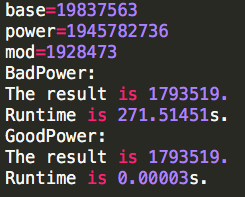
\includegraphics[height=7.09cm,width=8.82cm]{power.png}
\caption{两种模幂算法结果对比}
\label{img_power}
\end{figure}



\newpage{}
\section{中国剩余定理}
\subsection{中国剩余定理简述}
设整数$m_1, m_2, \cdots, m_n$两两互素,则对任意的整数$a_1, a_2, \cdots, a_n$,方程组
\begin{equation}
\left\{
     \begin{array}{lr}
     x\equiv a_1\quad (mod\  m_1)    \\
     x\equiv a_2\quad (mod\  m_2)    \\
     \quad \vdots \\
     x\equiv a_n\quad (mod\  m_n)    \\  
     \end{array}
\right.
\end{equation}
有同余意义下唯一解,且可如下构造:

设$$M = \prod_{i=1}^{n}{m_i},$$并设$M_i = M / m_i, \quad \forall i = 1,2,\cdots, n$。
设$M'_i$为满足$M'_iM_i \equiv 1 \quad (mod \  m_i)$的整数,则方程组的解为:
$$x\equiv \sum^{n}_{i = 1} M'_iM_ia_i \quad (mod\  M)$$
%\newpage{}
\subsection{算法实现}

\begin{algorithm}  
    \caption{中国剩余定理}  
    \begin{algorithmic}[1] %每行显示行号  
        \Require 余数表$remainders[]$, 模数表$mods[]$, 模数表积$modProduct$  
        \Ensure 解$root$  
        \Function {reverse}{$n, mod$}
            \State $gcd, coeN, coeMod \gets $\Call{extendEuclid}{$n, mod$}
            \State \Return coeN
        \EndFunction

        \Function {CRT}{$remainders, mods, modProduct$}   
            \State $root \gets 0$
            \For {each $i\in [1, len(mods)]$}
                \State $rest \gets modProduct / mods[i]$
                \State $rev \gets $\Call{reverse}{$rest, mods[i]$}
                \State $root \gets root + rev * rest * remainders[i]$
                \State $root \gets root \% modProduct$
            \EndFor
            \State \Return $root$
        \EndFunction  
    \end{algorithmic}  
\end{algorithm} 
CRT算法需要调用之前写过的扩展欧几里得算法,可获得数论倒数(逆元),就是算法中得到了$n$的系数。模数之积$modProduct$可以在输入时一并求出,故不在函数里给出,而是作为函数的参数给出。此外,本算法假设给出的模都是两两互素的。
\subsection{测试样例}
如图\ref{img_crt}所示,输入方程数和每个方程的余数及模,可求出方程的解,且用时很快。
\begin{figure}[htbp]
\centering
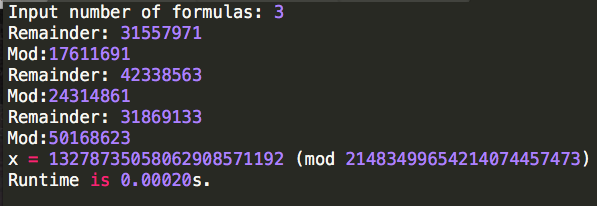
\includegraphics[height=4.12cm,width=11.94cm]{crt.png}
\caption{中国剩余定理测试}
\label{img_crt}
\end{figure}

\section{感想}
本次实验让我加深了对几个重要算法的理解,并且加强了python编程技术。在计算Eratosthenes筛法的时间复杂度时,我查阅了一些资料才计算出来,简单的算法的时间复杂度并不简单。

然而,在编写高效算法之前必须编写低效算法十分不合理。尤其是Eratosthenes筛法的低效算法(递归算法)其实根本就不存在,在wiki上也查不到,让我浪费了很多时间。我认为这些低效的过时算法应该被摒弃。对于更大的数,筛法业已十分低效,不再适合作为应用算法,所以没必要在此计较。

花费了很多时间完成本次实验和报告。功不唐捐。

\end{document}